\section{Optimal Control of Pitch and Travel with Feedback (LQ)}\label{sec:prob3}
This problem involves implementing an LQ controller for optimal control with feedback. We calculated a gain matrix K using the discrete algebraic riccati equation solver dlqr, implemented feedback on the helicopter, and discussed if MPC is a good alternative to LQR.

\subsection{Calculating the gain matrix K}
Feedback for the system is introduced by using $u_k=u_k^*-K^T(x_k-x_k^*)$. Here $x*$ is the optimal trajectory and $u*$ is the optimal input sequence. A good choice for K was found by minimizing the objective function:
\begin{equation}
J = \sum_{i=0}^\infty {\Delta x_{i+1}^TQ\Delta x_{i+1} + u_{i}^TRu_{i}}
\end{equation}
We used the built in MATLAB function dlqr to solve the riccati equation for the corresponding optimization problem and to compute the gain matrix K. 
This function depend on the system matrices A and B as well as Q and R. At first we chose Q and R to be:

\begin{equation}
\mathbf{Q} =
\begin{bmatrix}
1 & 0 & 0 & 0 \\
0 & 1 & 0 & 0 \\
0 & 0 & 1 & 0 \\
0 & 0 & 0 & 1
\end{bmatrix}
\qquad\mathbf{R}=1
\end{equation}

 By trial and error we got the best result by penalizing deviation in the travel trajectory relatively more than the pitch referance. This gave us a new Q matrix on the form:

\begin{equation}
\mathbf{Q} =
\begin{bmatrix}
50 & 0 & 0 & 0 \\
0 & 1 & 0 & 0 \\
0 & 0 & 1 & 0 \\
0 & 0 & 0 & 1
\end{bmatrix}
\end{equation}.


\subsection{Implementing feedback on the helicopter}
An implementation of feedback can be seen on the simulink diagram.

%Figure of simulink model with feedback
\begin{figure}[htb]
	\centering
   	 \makebox[\textwidth][c]{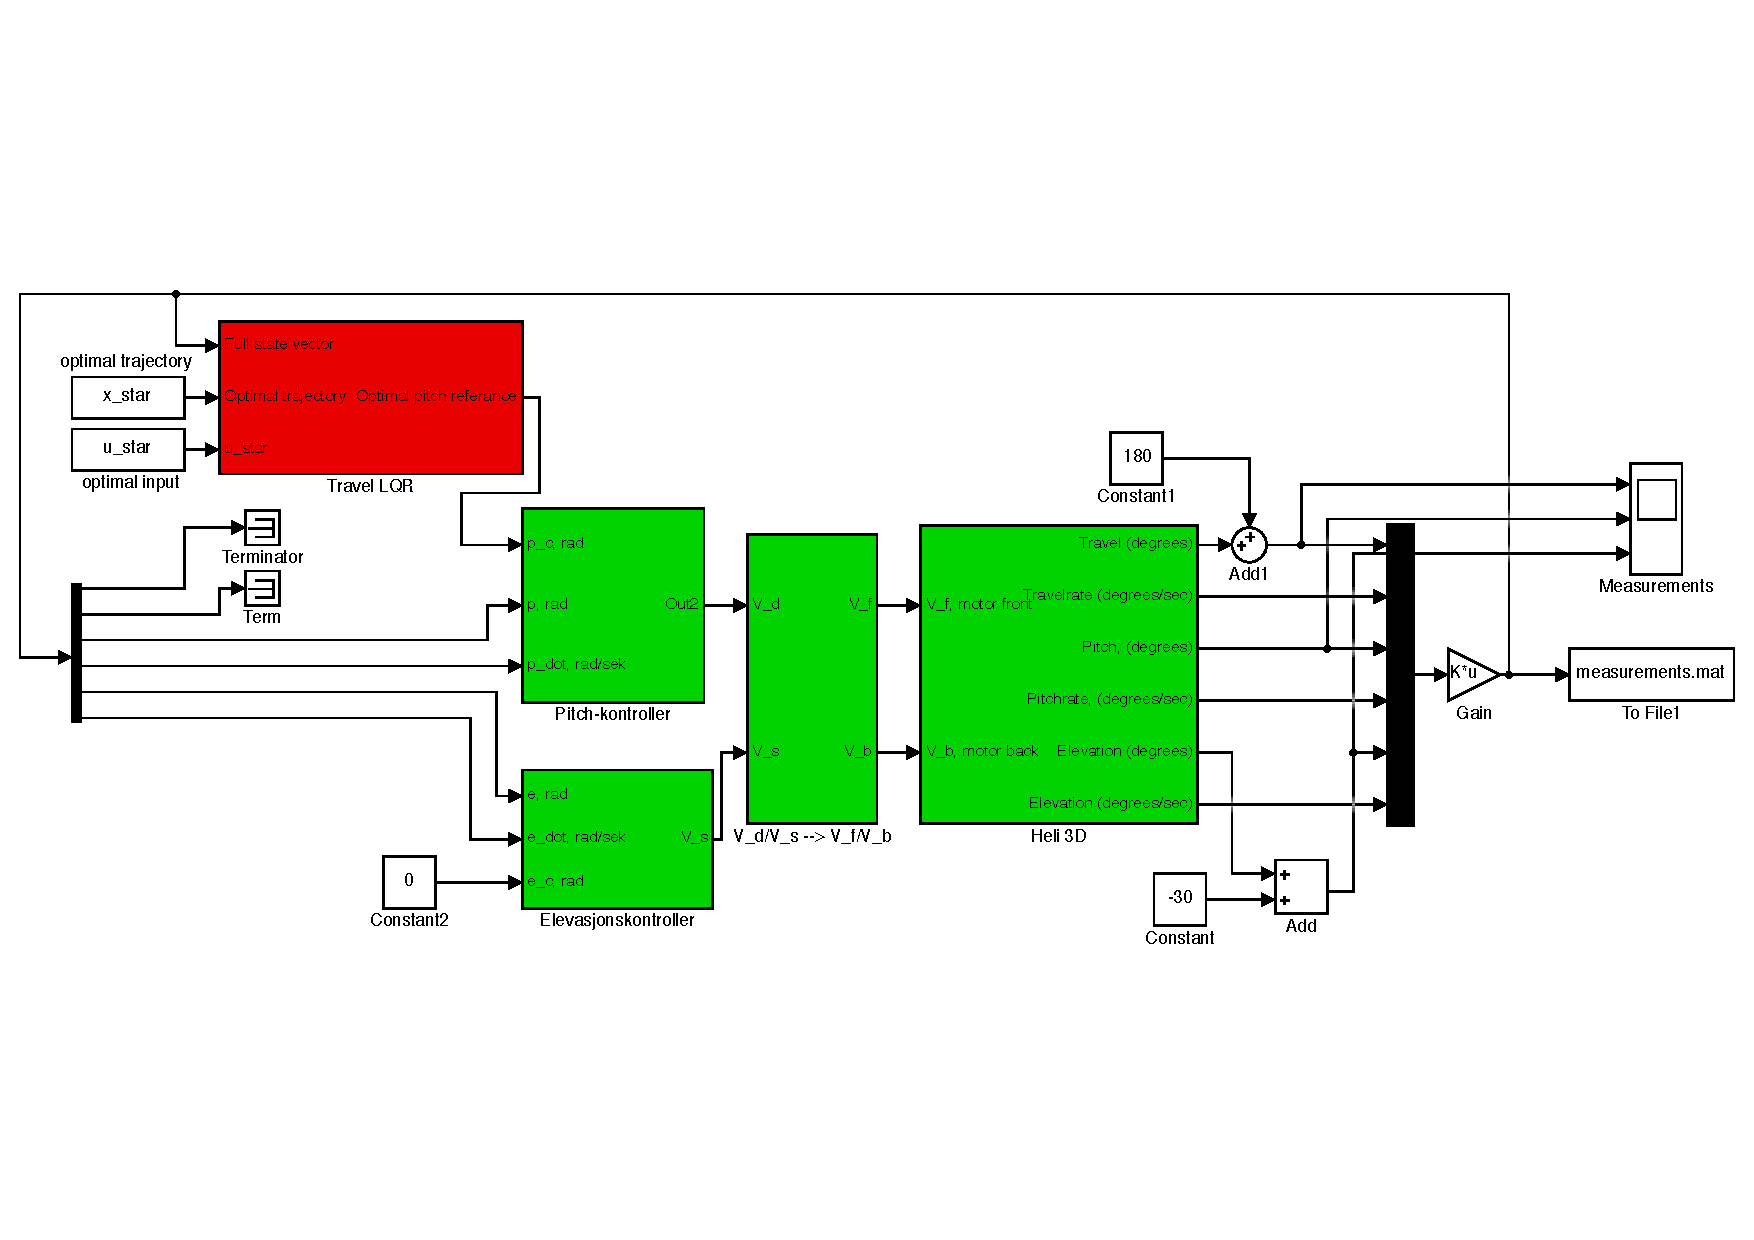
\includegraphics[width=1.2\textwidth]{figures/day3/day3_mdl}}
	\caption{Simulink model with feedback}
	\label{fig:day3_mdl}
\end{figure}

By using the gain matrix K calculated in last task, we see that by penalizing travel hard and pitch soft, the helicopter follows the travel trajectory closer than when weighting all states the same.
%Figure of helicopter response for Q_LQR = diag[50 1 1 1]
\begin{figure}[htb]
	\centering
    	\makebox[\textwidth][c]{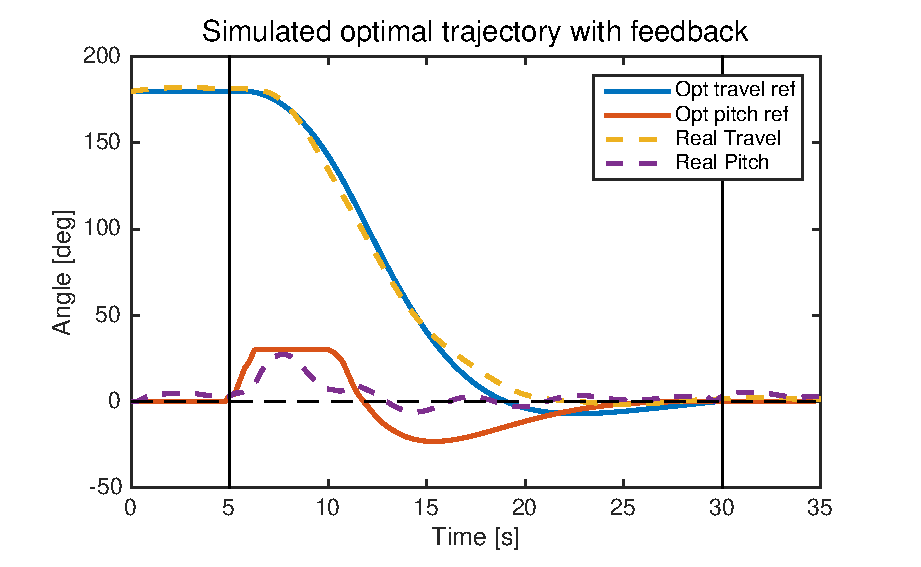
\includegraphics[width=1.2\textwidth]{figures/day3/plot_day3_q_50_1_1_1}}
	\caption{Plot of day 3 with Q = diag(50 1 1 1 )}
	\label{fig:day3_plot_50_1_1_1}
\end{figure}

We also tried penalizing the pitch more than travel, which gave us a bad result. Figure \ref{fig:day3_plot_1_1_10_1} shows how the real travel trajectory did not follow the optimal. This is because the optimal pitch reference trajectory is based on a bad model.
%Figure of helicopter response for Q_LQR = diag[1 1 10 1]
\begin{figure}[htb]
	\centering
    	\makebox[\textwidth][c]{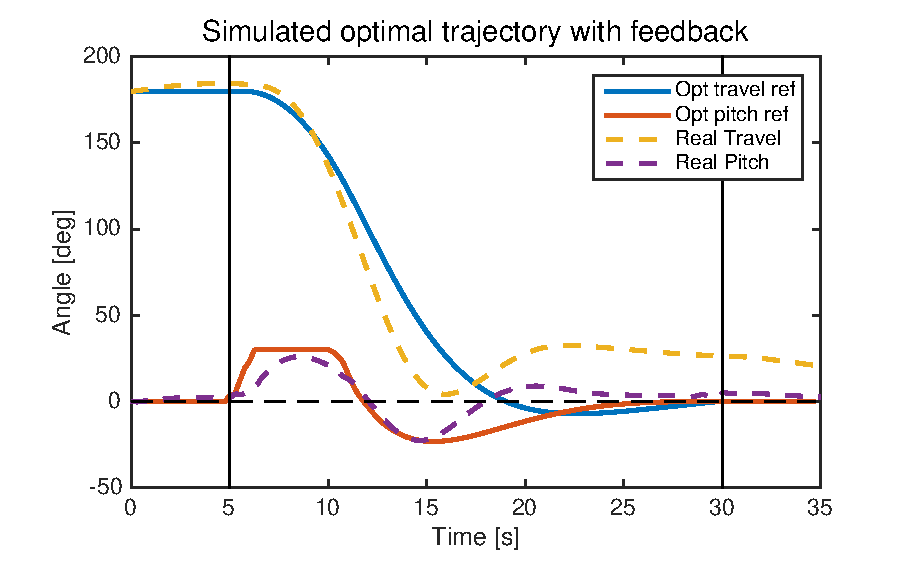
\includegraphics[width=1.2\textwidth]{figures/day3/plot_day3_q_1_1_10_1}}
	\caption{Plot of day 3 with Q = diag(1 1 10 1 )}
	\label{fig:day3_plot_1_1_10_1}
\end{figure}

\subsection{Comparison between LQR and MPC}
The way to implement an MPC controller would be to use the same procedure as for the LQR, but for every time step. Then using the first time step as the input u.

The advantages of using MPC instead of LQR; is that it gives us the possibility to have constraints in the regulator, can potentially produce a trajectory which performs its' task more cheaper and we get a implicit feedback with the use of MPC.
The main disadvantage of using MPC is that the calculations are a lot heavier to perform.
%Figure of figure 8, but with MPC implemented instead (if we have a figure of this)
